\chapter{Anexo. Manual de Instalaci�n OpenNI/OpenCV}

\section{Introducci�n}

El objetivo de este manual es explicar la instalaci�n del {\it driver OpenNi} y del {\it framework OpenCV}, para la utilizaci�n del dispositivo kinect, en cualquier equipo de c�mputo, en este documento se citan los requerimientos previos con los que el usuario debe contar.\\\\ 
Tambi�n se explican los pasos necesarios para una correcta instalaci�n.
El {\it driver y framework} son multiplataforma, con soporte para {\it Linux, Windows � Mac OS}.
Este manual s�lo describe el proceso de instalaci�n y configuraci�n para una distribuci�n de {\it Linux}. El manual incluye las versiones de los paquetes que se usaron, otras versiones pueden no funcionar, pero puede servir como previo para la b�squeda de informaci�n.
 
 
\section{Requisitos previos}

Tener instalada una distribuci�n de {\it Linux}. 
Este manual fue probado con {\it Ubuntu} $11$.$04$ en $32$ bits.

\subsection{Sistema Operativo}

En caso de no tener una distrubuci�n Linux los pasos b�sicos se pueden resumir en:
\begin{enumerate}
\item Se inserta el disco y se procede a instalar
\item Despu�s nos dar� una serie de opciones, de la cual usaremos la opci�n de algo mas
\item Se escoge la partici�n mas grande  con la que se cuenta y se reduce el espacio
\item Nos quedara un espacio libre, el cual fue reducido en la partici�n, este espacio se usara para crear una nueva partici�n.
\item Se crea la partici�n, que sea de tipo l�gica
\item Por �ltimo, se le da instalar y seguimos las instrucciones del asistente
\end{enumerate}

\subsection{Gestor de paquetes}

Las distribuciones incluyen gestores de paquetes (Figura \ref{fig:8.1}) que ayudan en la instalaci�n de bibliotecas de funciones,pero en caso de no tener un gestor instalador se pueden seguir los siguientes pasos:

\begin{enumerate}
\item Se abre una terminal.
\item Se escribe el siguiente comando:
\begin{verbatim}
sudo apt-get install synaptic
\end{verbatim}
\end{enumerate}

\begin{figure}[h1]
\centering
\includegraphics[scale=0.9]{maninstall/figura1Synaptic.ps} %[0cm,0cm][16.5cm,16cm]
\caption{gestor de paquetes.}
\label{fig:8.1}
\end{figure}

\subsection{Actualizaci�n de Repositorios}
Es necesario actualizar los repositorios(Figura \ref{fig:8.2}) de la distribuci�n, para saber si no faltan paquetes � si hay mejoras de algunos, para ello se siguen los siguientes pasos:
\begin{enumerate}
\item Se abre una terminal.
\item Se escribe el siguiente comando:
\begin{verbatim}
sudo apt-get update
\end{verbatim}
\end{enumerate}

\begin{figure}[h1]
\centering
\includegraphics[scale=0.9]{maninstall/figura2Update.ps} %[0cm,0cm][16.5cm,16cm]
\caption{actualizar repositorios.}
\label{fig:8.2}
\end{figure}

\subsection{Instalaci�n de Paqueteria}
Esto son parte de los paquetes que se debe instalar, para poder trabajar con el {\it drive} y el {\it API}. para ello se siguen los siguientes pasos:
\begin{enumerate}
\item Se abre una terminal.
\item Se escribe el siguiente comando(Figura \ref{fig:8.3}):
\begin{verbatim}
sudo apt-get install build-essential mercurial linux-headers-`uname -r`
\end{verbatim}
\end{enumerate}

\newpage
\begin{figure}[h1]
\centering
\includegraphics[scale=0.9]{maninstall/figura3BuildEssential.ps} %[0cm,0cm][16.5cm,16cm]
\caption{build-essential.}
\label{fig:8.3}
\end{figure}

Tambi�n se debe instalar {\it gcc, python, libusb, freeglut3, jdk, graphviz, mono, doxygen}
La forma que se puede instalar se puede checar directamente desde la p�gina de {\it OpenNI}, pero para facilitar la tarea, a continuaci�n se describen los comandos que se deben seguir:
 
\begin{enumerate}
	\item GCC 4.x\\
De: http://gcc.gnu.org/releases.html \\
O a trav�s de apt:
\begin{verbatim}
sudo apt-get install g++
\end{verbatim}

	\item Python 2.6 + / 3.x\\
De: http://www.python.org/download/ \\
O a trav�s de apt:
\begin{verbatim}
sudo apt-get install python
\end{verbatim}

	\item LibUSB 1.0.8\\
De: http://sourceforge.net/projects/libusb/ \\
O a trav�s de apt:
\begin{verbatim}
sudo apt-get install libusb-1.0-0-dev
\end{verbatim}

	\item freeglut3\\
De: http://freeglut.sourceforge.net/index.php download \\
O a trav�s de apt:
\begin{verbatim}
sudo apt-get install freeglut3-dev
\end{verbatim}

	\item JDK 6.0\\
De: http://www.oracle.com/technetwork/java/javase/downloads/jdk-6u26-download-400750.html \\
O a trav�s de apt:
\begin{verbatim}
sudo add-apt-repositorio "deb socio http://archive.canonical.com/ l�cido"
sudo apt-get update
sudo apt-get install sun-java6-jdk
\end{verbatim}

	\item Doxygen\\
De: http://www.stack.nl/ ~ dimitri / doxygen / download.html  latestsrc \\
O a trav�s de apt:
\begin{verbatim}
sudo apt-get install doxygen
\end{verbatim}

	\item GraphViz\\
De: http://www.graphviz.org/Download\_linux\_ubuntu.php\\
O a trav�s de apt:
\begin{verbatim}
sudo apt-get install graphviz
\end{verbatim}

	\item Mono\\
De: http://www.go-mono.com/mono-downloads/download.html\\
O a trav�s de apt:
\begin{verbatim}
sudo apt-get install mono-complete
\end{verbatim}
\end{enumerate}

\section{Instalaci�n de OpenNI y OpenCv}
\subsection{Pasos para la instalaci�n de OpenNI}

Paso 1  Descargue los archivos desde el siguiente link:\\ http://www.openni.org/Downloads/OpenNIModules.aspx\\\\

Se recomienda que use estos paquetes(Cuadro \ref{tab:8.1}):
\begin{table}[h]
\centering
\begin{tabular}{|c|c|}%{|p{4.8cm}|p{11cm}|}
\hline
Paquete & Versi�n\\ \hline
OpenNI & openni-bin-dev-linux-x86-v1.5.2.23\\ \hline
Nite & nite-bin-linux-x86-v1.5.2.21\\ \hline
Sensor & sensor-bin-linux-x86-v5.1.0.41\\ \hline
SensorKinect & avin2-SensorKinect-faf4994 (Version 5.1.0.25 version - Dec 18th 2011)\\ \hline
\end{tabular}
\caption{Paquetes de OpenNI.}
\label{tab:8.1}
\end{table}

Todos los paquetes deben ser versiones estables, en la siguiente Figura \ref{fig:8.4} se muestra como se visualiza la p�gina, as� mismo  estos son los nombres con los que encontraremos los paquetes {\it openni, nite y sensor}:
\begin{itemize}
	\item Openni - OpenNI Binaries
	\item Nite - OpenNI Compliant Middleware Binaries
	\item	Sensor - OpenNI Compliant Hardware Binaries
\end{itemize}

\newpage
\begin{figure}[h1]
\centering
\includegraphics[scale=0.9]{maninstall/figura4DescargasOpenni.ps} %[0cm,0cm][16.5cm,16cm]
\caption{Pagina de Descargas de OpenNi.}
\label{fig:8.4}
\end{figure}

\begin{itemize}
    \item Hacer una nueva carpeta llamada Kinect (Figura \ref{fig:8.5}).
\begin{verbatim}
$ cd
$ mkdir Kinect
$ cd Kinect
\end{verbatim}
\end{itemize}

\begin{figure}[h1]
\centering
\includegraphics[scale=0.9]{maninstall/figura5CarpetaKinect.ps} %[0cm,0cm][16.5cm,16cm]
\caption{Crear carpeta Kinect.}
\label{fig:8.5}
\end{figure}
